\documentclass[usenatbib]{mnras}
%\documentclass[]{mnras}
%\documentclass[letterpaper]{mnras}
%\voffset=-0.6in %only for arXiv

%\usepackage{newtxtext,newtxmath} %for smaller font in MNRAS, ignored on arXiv
%\pdfminorversion=5 %only for MNRAS
\usepackage{multirow}
\usepackage{rotating}
\usepackage{graphicx}
\usepackage{booktabs}
\usepackage{textcomp}
\usepackage{pbox}
\usepackage{natbib}
\usepackage{mathtools}
\usepackage{gensymb}
\usepackage{colortbl}
\usepackage{color}
%\usepackage{xcolor}
\usepackage{amssymb}
\usepackage{amsfonts}
\usepackage{verbatim}
\usepackage{scalefnt}
\usepackage[percent]{overpic}
\usepackage[T1]{fontenc} %only for MNRAS
\usepackage{aecompl} %only for MNRAS
\usepackage{ulem}
\usepackage{cleveref}
\usepackage{todonotes}
%\usepackage[utf8]{inputenc}
\usepackage[english]{babel}
\usepackage{siunitx}
\usepackage{pbox}
\usepackage{float}
\usepackage{lineno}
\usepackage{enumitem}
\usepackage{tikz}
\usepackage{tikz-3dplot}
\usetikzlibrary{angles, quotes}
\usepackage{tkz-euclide}
\usetkzobj{all}
\usepackage{subcaption}
\usepackage{multicol}
\usepackage[]{threeparttable}

\setcounter{topnumber}{2} %default 2, current 3
%\setcounter{bottomnumber}{3} % default 1, current 3
%\setcounter{totalnumber}{3} % default 3, current 3
\renewcommand{\topfraction}{0.9} % default 0.7, current 0.85
%\renewcommand{\bottomfraction}{0.9} % default 0.3, current 0.85
%\renewcommand{\textfraction}{0.15} % default 0.2, current 0.15
\renewcommand{\floatpagefraction}{0.9} % default 0.5, current 0.7
\renewcommand{\dbltopfraction}{0.9} %current 0.9

\def\msun{~{\rm M}_\odot}
\def\lsim{\mathrel{\rlap{\lower 3pt \hbox{$\sim$}} \raise 2.0pt \hbox{$<$}}}
\def\gsim{\mathrel{\rlap{\lower 3pt \hbox{$\sim$}} \raise 2.0pt \hbox{$>$}}}

%Not needed any longer; left here as an example for future missing journals
%\newcommand{\aj}{AJ}% Astronomical Journal

\newcommand{\comments}[1]{} %usage: \comments{}
\newcommand{\TD}[1]{\textcolor{magenta}{\bf [To do] #1}}
\newcommand\bncomment[1]{\textcolor{green}{BN: #1}}
\newcommand\T{\rule{0pt}{2.6ex}}       % Top strut
\newcommand\B{\rule[-1.2ex]{0pt}{0pt}} % Bottom strut
\newcommand{\Vector}[1]{\mathbf{#1}}
\newcommand{\sub}[1]{_{\text{#1}}}


\title{Empirical structure models of  Jupiter}

\author[]{{Benno A. Neuenschwander}$^{1}$,
{Ravit Helled}$^{1}$
{Naor Movshovitz}$^{2}$,
{Jonathan Fortney}$^{2}$
\\
% List of institutions
$^{1}$Center for Theoretical Astrophysics and Cosmology, Institute for Computational Science, University of Zurich, \\Winterthurerstrasse 190, CH-8057 Z{\"u}rich, Switzerland\\
$^{2}$Astronomy and Astrophysics, University of California, Santa Cruz, \\ ISB 119, Science Hill, Santa Cruz, California, USA\\
}

\date{Accepted XXX. Received YYY; in original form ZZZ}

\pubyear{2020}

\begin{document}

\label{firstpage}

\pagerange{\pageref{firstpage}--\pageref{lastpage}}

\maketitle

%%%%%%%%%%
%%%%%%%%%%
%Abstract%
%%%%%%%%%%
%%%%%%%%%%

\begin{abstract}
\TD{make it new}
Knowledge of Jupiter's internal structure is key to understand its formation and evolution. 
Interior models of Jupiter that fit Juno's measured gravitational field suggest an inhomogeneous interior and the existence of a diluted core. (heavy elements distributed in H and He => uncertainty in modeling these region). These 
models, however, strongly depend on the model assumptions and the used Equation of State (EoS). 
%As under Jupiter's interior conditions EoS are hard to measure/verify experimentally, significant uncertainties may arise.  
%But EoS are often extrapolated or are emerging simulations to be applicable on conditions in Jupiter's interior, leading to large uncertainties. 
A complementary approach is to use empirical structure models where no underlying physics is assumed. 
These models can reveal new insights on the planetary interior and then be compared to standard models. 
%that can It is therefore desirable to compare these results to empirical internal models.
First we investigate Jupiter's interior by converging density profiles, composed of three polytropes and calculated with Theory of Figures 4$^{\text{th}}$ order, to the measured second and fourth gravitational coefficient $J_2$ \& $J_4$. 
%{\bf The abstract needs a lot of work....
First, we present new empirical models of Jupiter using three polytropes where the gravitational coefficients are calculated with a 4$^{\text{th}}$ order Theory of Figures. We next investigate the MoI-J$_2$ connection, the limitation of assuming a constant density core...  finally, we... We conclude that...
%By varying the innermost polytrope's mass and size the effect of different core properties on the normalized moment of inertia (MoI) is studied.
We conclude that a MoI with a accuracy of $\approx0.2\%$ can be used to further constrain Jupiter's core properties. 
%\bf{By applying \citet{2017Wahl} MoI range, we predict Jupiter to have a core with $0.15 \lsim{r\sub{core}} \lsim{0.3}$ and $25 \text{ M}_\oplus \lsim{m\sub{core}} \lsim{40\text{ M}_\oplus}$.} 
%We conclude that measuring Jupiter's moment of  inertia (MoI) with accuracy of  $\approx0.1\%$ can be used to further constrain Jupiter's core properties. By applying the MoI range proposed by \cite{2017Wahl} we predict Jupiter to have a core with $0.15 \lsim{r\sub{core}} \lsim{0.3}$ and $25 \text{ M}_\oplus \lsim{m\sub{core}} \lsim{40\text{ M}_\oplus}$. This stands in direct contradiction with their results and needs further investigations. \\
We also investigate under which conditions a compressed core can be simplified by a constant density core.  %We suggest to not model Jupiter's core as a constant density core for $r\sub{core}\gsim{0.2}$.
%Further investigations suggest for Jupiter to not have a constant density core with a size exceeding $r\sub{core}=0.2$.
\end{abstract}

\begin{keywords}
\TD{Keywords}
%gravitational waves -- methods, polarization, telescopes; \;
%techniques -- interferometric; \;
%stars --  CD$-30^\circ$ 11223; \;
%subdwarfs -- tidal effects \;
\end{keywords}

%%%%%%%%%%%%%%
%%%%%%%%%%%%%%
%Introduction%
%%%%%%%%%%%%%%
%%%%%%%%%%%%%%

\section{Introduction}\label{sec:introduction}
%The giant planets in the Solar System incorporate a lot of unsolved questions. Until present day their formation process remains unknown, as well as the distribution of elements which are heavier than helium (usually called "heavy elements"). It is unrevealed whether their heavy elements are settled in their center to form a core or whether they are (partially) mixed or dissolved in hydrogen (H) and helium (He) within the mantle. Both scenarios raise continuative questions about the eventual core size and mass, or how and how much the heavy elements are mixed within the envelope. But these answers are crucial to understand the genesis and evolution of giant planets.}
Understanding the internal structure of Jupiter is a longstanding objective in planetary science. 
Research on planetary interiors goes back a few decades (e.g., \cite{Podolak1974, Decampli1979}).
As more accurate data is collected planetary modelers aim to further constrain the planetary bulk composition, as well as the distribution of the different chemical elements inside the planet.
The planetary internal structure cannot be observed directly. Information about the composition and its depth dependence is inferred by fitting theoretical models to the available data.

Structure models are designed to reproduce the measured planetary mass, radius and gravitational field. 
%The gravitational field (moments), which are typically measured by Doppler tracking a space probe. 
For Jupiter, the ongoing Juno mission has provided accurate measurements of its gravity field via Doppler tracking \citep{NatureIess, Folkner2017, Bolton2017}.
\par

The total potential $U(\Vector{r})$ in the co-rotating reference frame of a planet consists of its gravitational potential $V(\Vector{r})$ and centrifugal potential $Q(\Vector{r})$. Assuming the planet is symmetric along its rotation axis one can write the total potential in the following form:
\begin{align*}
    U(r, \theta) &= V(r, \theta) + Q(r, \theta) \\
    &= -\frac{GM}{r} \left(J_0P_0-\sum_{n=1}^{\infty}\left( \frac{a}{r}\right)^n J_n P_n(\cos\theta)\right) \\
    &\quad\text{ }+ \frac{1}{2}\omega^2r^2\sin^2(\theta),
\end{align*}
where $r$ and  $\theta$ are the distance and co-latitude, respectively, $G$ the gravitational constant, $M$ the planet's mass, $a$ the equatorial radius, $P_n(\cos\theta)$ the corresponding Legendre Polynomials and $\omega$ the rotation period. The coefficients $J_n$ are integrals over the planet's volume of the mass distribution $\rho(\Vector{r})$ requiring knowledge of the planet's shape, itself determined by the potential. An iterative solution process converges to the self-consistent equilibrium shape and gravity. For a fluid planet in hydrostatic equilibrium ($U(r, \theta) = const.$), only the even order coefficients $J_{2n}$ are non-zero. 
%Usually only the even indices are considered, as the north and south hemispheres are symmetric in first order (as used in e.g. \cite{Liu2008}), and hydro-static equilibrium is assumed ($U(r, \theta) = const.$) (e.g. \cite{Guillot2014}). 

Figure \ref{fig:contr_function} illustrates the contribution functions of the first four even $J$-values for Jupiter, similar as in e.g. \citet{2011Helled}.
Note that the maximal contribution is increasing with the order of $J_{2n}$ and that the higher-order gravitational coefficients are more sensitive to the outermost region of the object. $J_0$ is corresponding to the object's mass.
\begin{figure}
    \centering
    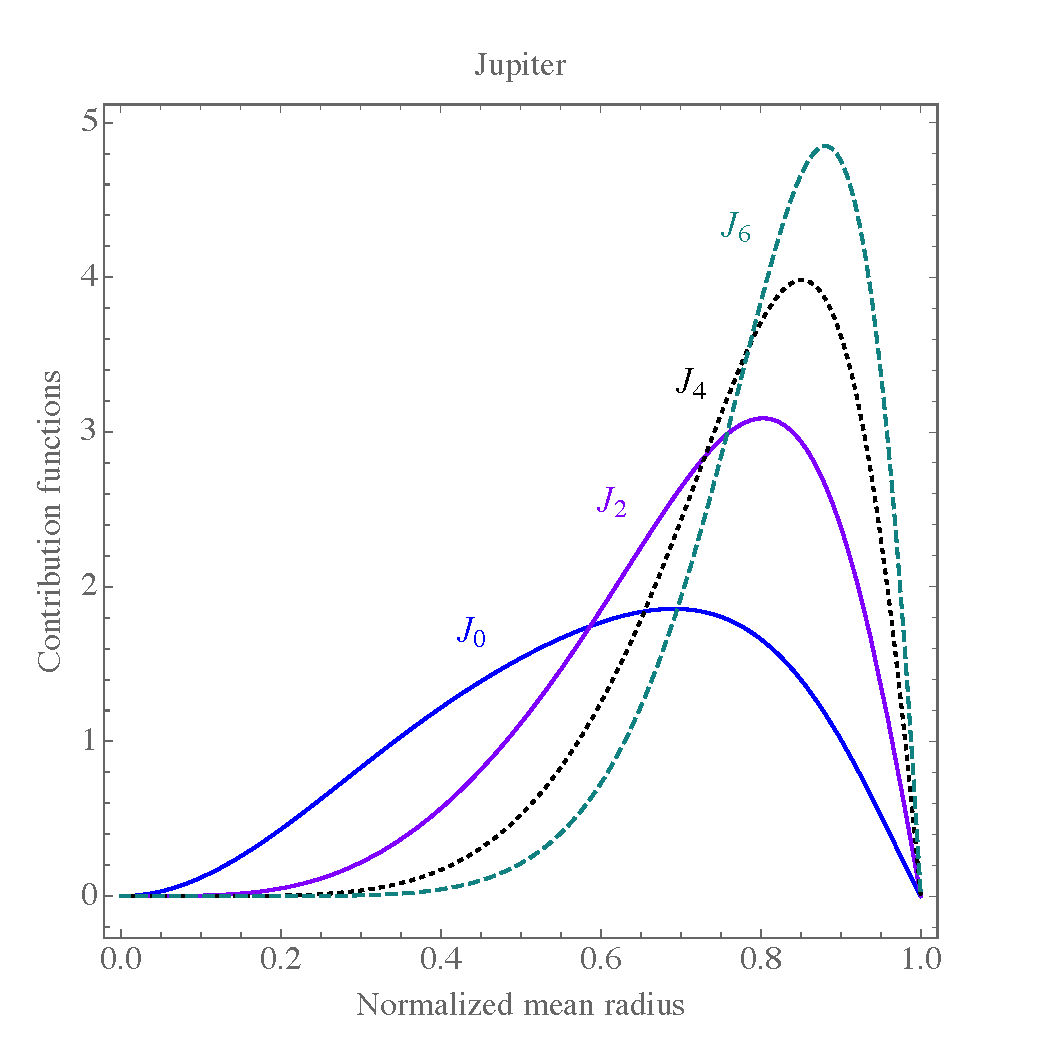
\includegraphics[width = 0.5\textwidth]{Figures/CF_4Benno.pdf}
    \caption{Contribution functions of selected $J_{2n}$-values depending on Jupiter's mean radius. Contribution functions are the normalized integrands of the gravitational moments and describe how different layers contribute differently to the $J_{2n}$ (\cite{ZHARKOV1974, Guillot2009}). The higher order coefficients are more sensitive to the outermost region of the planet and have a higher maximum contribution. Note that $J_0$ corresponds to the mass.}
    \label{fig:contr_function}
\end{figure}

Our understanding of Jupiter's interior has been challenged by Juno's measurements. 
Models reproducing the new data suggest that Jupiter's interior is inhomogeneous and display an extended core-mantle transition in the deep interior rather than a sharp boundary with a central solid core \cite{2017Wahl, Debras_2019}. 
This result, if correct, has important implications. 
First, it challenges the common view of a three-layered planet consisting of a distinct core, mantle and envelope. 
Second, it suggests that the deep interior of the planet should be modeled accounting for the presence of hydrogen and helium and possibly, composition gradients.
Finally, this more complex internal structure must be explained by formation and evolution models of the planet (e.g. \cite{HelledStevenson2017, Vazan2018, Muller2019}).   

It should be noted, however, that these recent internal structure models of Jupiter depend strongly the equation of state (EoS) of the assumed composition; in particular the EoS of hydrogen at a wide range of pressure and temperature. 
Although our understanding of the hydrogen EoS has been significantly improved in the last decade, the EoS is still not perfectly known. In addition, further complexities arise from possible phase transitions and the behaviour of mixtures. Lastly, the composition still has to be \emph{assumed} by the modeler, potentially leading to additional uncertainties and biases.
While structure models that are based on physical EoSs generate detailed and easy to interpret models of Jupiter's composition and its depth dependence, there is also clear value in taking a complementary approach where the density profile is generated with a mathematical function, without direct reference to composition (e.g. \cite{Helled2009,Helled2011_jup, Movshovitz2019, Ni2018}).
A convenient approach is to use empirical density profiles based on mathematical polytropes (\cite{Hubbard1975, Movshovitz2019}).
A polytrope describes the relation between the pressure $P$ and the density $\rho$ according to the parameters $n$ and $K$: 
\begin{equation}
    P = K\rho^{1+\frac{1}{n}}.
    \label{eq:polytrope}
\end{equation}
Despite the simplicity of the function, it was found that polytropes can represent Jupiter's interior rather well (\cite{Hubbard1975, Hubbard1999}). \\ %H and He to a good extend but fail to describe heavy elements found in the core region. \\ 

Using gravitational data to describe and constrain a planet's interior yields non-unique solutions. In particular, it is hard to constrain the innermost region of a planet since the $J_{2n}$-values are "blind" to this part of the planet as shown in figure \ref{fig:contr_function}. \\

In this paper we aim to address the following questions: (1) Is it possible to put some limits on Jupiter's core properties using only an accurate measurement of $J_2$ and $J_4$? And (2) Is there additional usable information in the moment of inertia (MoI) of the planet, that is not hopelessly degenerate with $J_2$ and $J_4$? %Could such additional information potentially constrains Jupiter's core? \\ 

In order to answer these questions we construct a large range of density profiles for Jupiter. In particular, we focus on the innermost region that can be viewed as representing the ``core''.  We next investigate the sensitivity of the inferred MoI, $J_2$ and $J_4$ values to the assumed core properties.
We also explore under what conditions assuming a constant density core (CDC) for Jupiter is appropriate. This consideration is crucial as structure models often assume a CDC rather than a compressed one (e.g. \cite{HELLED2011440}, \cite{Hubbard_2016}, \cite{Ni2018}, \cite{Debras_2019}). This assumption may be inappropriate for compressible materials. 
%physically not correct, as the density of material changes with pressure and temperature. 
We set an upper limit for the core radius of Jupiter for which the simplified CDC assumption does not affect the results for a given calculation method.

Our paper is organized as follows. In section \ref{sec:methods} we explain the calculation method and the characteristics of our models. In section \ref{sec:results} we present and discuss the resulting density profiles and the impact of a CDC. Finally we conclude with a summery and discussion of followup research in section \ref{sec:summary}.

\section{Methods} \label{sec:methods}
Density profiles of Jupiter are generated to fit the measured second and fourth gravitational coefficient $J_2$ \& $J_4$, as well as its mass, equatorial radius, and rotation period. Table \ref{tab:jupiter_properties} summarizes the planetary properties used for these models. 

Although Jupiter's interior can be represented fairly well with a single polytrope (e.g. \cite{Wisdom_2016, Hubbard1975}), in order to explore a larger possible parameter space we consider density profiles represented by (up to) three polytropes. This accounts for a possible distinct core (as predicted by the core accretion model, e.g., \citet{Pollack1996}), and a possible sharp transition where molecular hydrogen becomes conductive due to pressure (e.g. \cite{Nellis2000, Helled2018}). Nevertheless this might be one of the most constraining assumption made. %as \cite{Debras_2019} suggest to encompass at least four different regions (a compact core followed by a diluted core region and an inner and outer envelope). \\ {\bf but then shouldn't we use 4??}

The three polytropes create three distinct regions in the planet, but these are different from traditional three-layer models in that these are not necessarily regions of homogeneous composition. Solutions with consolidated polytropes (as e.g. potentially observed for diluted cores) leading to fewer density jumps are permitted.

The innermost polytrope is designated as ``core'' but in our models it should not be interpreted as a standard pure rock and/or ice core. First, since these are empirical density profiles, the different regions do not necessarily represent different compositions.
Second, the innermost polytrope is not supposed to describe a compact core in the traditional sense. It is solely describing the \textit{innermost region}. 

We calculate gravity coefficients from th density profiles using 4$^{\text{th}}$-order Theory of Figures (ToF). ToF is based on the theoretical framework of \cite{ZharkovVladimirNaumovich1978Popi} and is also described in \cite{Zharkov1970, Zharkov1975, Hubbard2014,Nettelmann_2017}. 
It is applicable on fluid planets in hydrostatic equilibrium with uniform rotation. 
ToF therefore neglects odd gravitational coefficients ($J_{2n+1}=0$) and does not account for differential rotation or dynamical effects. To first order Jupiter is in hydrostatic equilibrium (e.g. \cite{Guillot2014}).
However, Jupiter's winds are expected to penetrate 3000 km deep into the planet and influence the density distribution (\cite{Kaspi2018}). This not only affects the $J_{2n+1}$ but also $J_{2n}$. We account for these effects by considering larger uncertainties in the measured $J$-values compared with the formal measurement errors (table \ref{tab:jupiter_properties}). %Because ToF only considers uniform (i.e., solid-body) rotation, the effects of the winds are incorporated by an enlarged formal uncertainty in the J-values (table \ref{tab:jupiter_properties}). 

ToF resolves the planet's shape on a finite set of equipotential levels. The more levels are evaluated, the more precisely the planet's continuous interior is approximated. Our models include 4096 equally spaced radius levels. The shape equations are evaluated on every $32^{nd}$ level and the solved shape functions are spline-interpolated in the radial direction between these levels. This speeds up the calculation significantly while maintaining the desired precision. We validate this method by comparison with previously published results
\citep{Nettelmann_2017}. 

%{\bf We want to do XXXX therefore we do XXXX}\\
We want to produce density profiles for a large range of core properties ($m\sub{core}$ and $r\sub{core}$) that fit Jupiter's measured mass, equatorial radius, rotation rate, $J_2$ and $J_4$. To assure a large variety of core properties, discrete ranges of core radii and masses are defined. Then each core instance, consisting of a radius $r_{\text{core}, i}$ and mass $m_{\text{core}, i}$, is investigated.
For each given core instance, polytrope parameters $K_{i}$, $n_i$ and $r\sub{trans}$ (the transition radius between the mantle and envelope polytrope) are found such that the resulting equilibrium gravity matches the measured $J_2$ and $J_4$ (we will call such models \textit{good results}). If values for the polytrope parameters cannot be found such that $J_2$ and $J_4$ are matched within their uncertainty, we exclude these core properties. 
%Otherwise profiles are called \textit{good results}. 
The search for model parameters is carried out by the simplex optimization algorithm \citep{Lagrias1998} \footnote{implemented by MATLAB's fminsearch} which is designed to find a local minimum only. It is thus not guaranteed that our models are the only, or even the best possible three-polytrope representations, only that they are valid ones.

We consider a core size range of $r\sub{core} = [0.025, 0.5]$ Jupiter radii, and a core mass range of $m\sub{core} = [1, 100] \text{ M}_{\oplus}$. This allows for solutions representing both the compact core and diluted core ideas.
The core mass is changed in steps of $1 \text{ M}_\oplus$ and the core radius in steps of $0.025$ (or 2.5\% of the planet's radius). Some extreme pressure profiles are excluded by restricting the central pressure to 100~Mbar \citep{Miguel2016,Debras_2019, 2017Wahl}. 
Further the central density is restricted to $\rho < 30,000$~kg/m$^3$ \citep{Helled2011_jup, Ni2018}, which is well above the expected density of rock at this pressure \citep{sesame7100, Musella2019,Thompson1974}.

\begin{threeparttable}
    \renewcommand\TPTminimum{\linewidth}
	\caption{Physical properties of Jupiter and its gravitational harmonics. $m\sub{rot}= \omega^2s^3/GM$ is the small parameter used by ToF, where $\omega$ is the angular velocity and $s$ the mean radius.}
	\begin{tabular}{l|ll}
			& \multicolumn{1}{c}{\textbf{Jupiter}} \\
		    \midrule
		Mass \tnote{1}		 	    & 317.8	     & [$M_\oplus$]\\  
		Equatorial radius \tnote{1}			& 71,492     & [\text{km}]\\ 
		%density \tnote{1}		 	& 1326 	     & [$\text{kg/m}^3$]\\  
		%Sun distance \tnote{1}	 	& 778.6      & [$\times10^6\text{ km}$]\\  
		%orbital period \tnote{1}    & 4331       & [$\text{days}$]\\
		Rotation period \tnote{2}	& 35,729.7	 & [$\text{s}$]\\ 
		%mean temperature \tnote{1}  & -110       & [$\degree \text{C}$]\\
		$J_{2}$ \tnote{3}			& 14,696.572 & $[\times10^6]$\\ 
		$J_{4}$ \tnote{3}			& -586.609 & $[\times10^6]$\\ 
		$\Delta J_{2,\text{formal}}$ \tnote{3} & 0.014	 & $[\times10^6]$\\  
		$\Delta J_{2,\text{winds}}$ \tnote{4}  & 0.568  & $[\times10^6]$\\
		$\Delta J_{4,\text{formal}}$ \tnote{3} & 0.004	 & $[\times10^6]$\\  
		$\Delta J_{4,\text{winds}}$ \tnote{4}  & 0.2257  & $[\times10^6]$\\
		$m\sub{rot}$                   & 8.340783   & $[\times10^2]$\\
	\end{tabular} 
	\begin{tablenotes}
	    \item[1] https://nssdc.gsfc.nasa.gov/planetary/factsheet/index.html 
	    \item[2] \cite{RIDDLE1976}
	    \item[3] \cite{NatureIess}
	    \item[4] \cite{Kaspi2018}
	\end{tablenotes}
	\label{tab:jupiter_properties}
\end{threeparttable}


\section{Results - New empirical Models} \label{sec:results}
Figure \ref{fig:all_in_one_MoI} (left panel) shows all investigated density profiles that fit Jupiter's measured gravity field. Color indicates MoI value. For comparison, three previously published Eos-bsaed models are overlaid, the solid black line is the model of \citet{Debras_2019} and the black dashed and dotted lines are solutions from \cite{2017Wahl} and \citet{Miguel2016}, respectively. Our polytropic models are in good agreement with the external density profiles, as they mark a subset of our solutions. Our piecewise-polytrope solutions include ones with lower central densities, potentially corresponding to a diluted core scenario, as well as ones with sharp transitions to a central region of high density, implying compact and presumably rocky cores.

We find that variations in the core properties mostly affect the outermost region ($r \gtrsim 0.75$), leaving the intermediate deep interior ($r \approx 0.35-0.75$) relatively unaffected, and therefore rather well-determined. 

Further the color trend shows that diluted cores with lower core densities have smaller MoI values compared to distinct and compact ones. This indicates that a precisely measured MoI value could further constrain Jupiter's interior. 

Although we put no limits on the value of $r\sub{trans}$, it is found that in most of the models where a large density jump occurs in the envelope, the transition radius is found at $r\sub{trans} \approx 0.75-0.9$ with a density around $\rho\sub{trans} \sim 250 -1500~\text{kg/m}^3$.

A detailed analysis of the constraining power of the MoI with respect to $J_2$ and $J_4$ is done in subsection \ref{subsection:MoI_vs_J2} and \ref{subsection:MoI_vs_core}. A closer look at the $P_{1,2}$ transition characteristics is taken in subsection \ref{subsection:Transition_behavior}. Then, a comparison to polynomial-based density profiles is shown in \ref{subsection:comparison_to_polynomials}. The impact of the model resolution (number of equipotential levels) on the $J$-values and the MoI is investigated in subsection \ref{subsection:resoltution_dependence}. Finally the effect of a simplified constant density core on the MoI and the gravitational coefficients is investigated in \ref{subsection:CDCvsPC}.

\begin{figure*}
    \begin{subfigure}{.5\textwidth}
    \includegraphics[width = 1\textwidth]{Figures/jupiter_figure_cut_off_MoI.pdf}
    \end{subfigure}%
    \begin{subfigure}{.5\textwidth}
    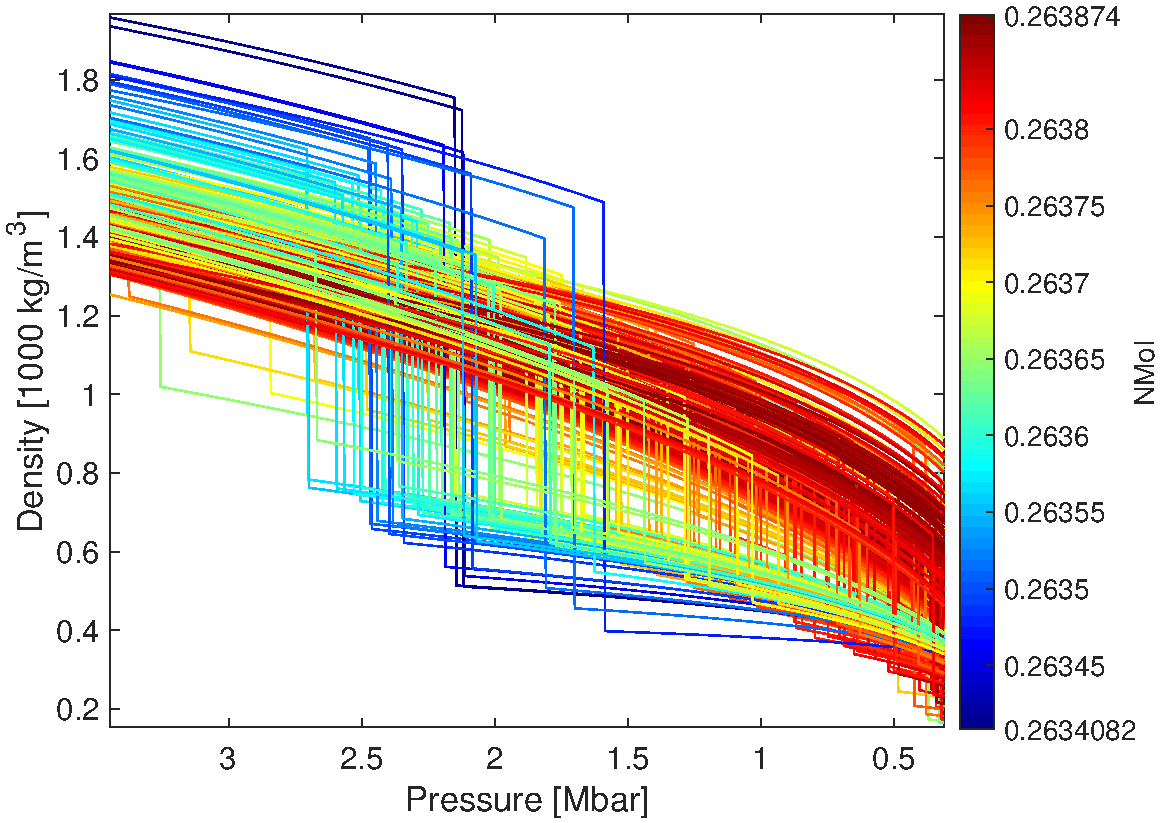
\includegraphics[width = 1\textwidth]{Figures/jupiter_all_in_one_rho_of_P_J4.pdf}
    \end{subfigure}
    \caption{\textbf{Left panel:} The density profiles of all \textit{good results} depending on the normalized mean radius. The color of each solution illustrates its MoI value. Results of \cite{Debras_2019}, \cite{2017Wahl} and \cite{Miguel2016} are represented by the black solid, black dashed and black dotted line, respectively. Core changes mainly affect the outer regions $r \gsim{0.75}$. Most density discontinuities in the envelope, while not forced, tend to occur between $r\sub{trans} \approx 0.75-0.9$. Further it shows a clear color trend, where diluted cores with a lower maximum core density have smaller MoI values with respect to rather distinct and compact ones. \\
    \textbf{Right panel:} The density profiles of all \textit{good results} depending on the transition pressure at the density discontinuity in the envelope. The color represents the solution's MoI value. Again some color trend is observable: Diluted cores with low MoI values have a transition pressures between $P\sub{trans} \approx 1.5 - 2.7$~Mbar. Accordingly, lower transition pressures are coupled to higher MoI values and more compact cores. An accurately measured MoI can further constrain transition properties as the transition density, radius and pressure.
    These density discontinuities can be interpreted either as He-rain and/or as phase transition from molecular to metallic hydrogen.} 
    \label{fig:all_in_one_MoI}
\end{figure*}

\subsection{Relation between the gravitational moments and the MoI} \label{subsection:MoI_vs_J2}
The MoI and the second gravitational moment $J_2$ are closely correlated, both involving similar integrals over the density profile. The Radau-Darwin relation \citep[e.g.][]{Helled2011_jup} is a useful approximation:
\begin{equation}
    \text{MoI}= \frac{2}{3} \left[ 1 -  \frac{2}{5} \left( \frac{5m\sub{rot}}{m\sub{rot}+3J_2} -1 \right)^{1/2} \right].
    \label{eq:RadauDarwin}
\end{equation}
However, it has been suggested by several studies that because MoI is not perfectly isomorphic with $J_{2}$ (or indeed with the gravity field in general) an \emph{independent} measurement of the MoI could be used to further constrain a planet's interior (e.g. \cite{HELLED2011440}).

Figure \ref{fig:jupiter_area_plotting_MoI} shows the relationship between MoI, core size, and core mass, in our piecewise-polytrope models.
%For each discrete core combination $r\sub{core}$ \& $m\sub{core}$, a color code represents the value of the solution's MoI. 
For many combinations of core properties either no \textit{good result} is found or the solution is excluded because it exceeds $P\sub{max}$ or $\rho\sub{max}$ (see section \ref{sec:methods}). Note that especially for small and heavy and for large and light cores no \textit{good results} are found. This is fairly intuitive, the former combination gets restricted by $\rho\sub{max}$ and the latter might produce negative density jumps at the core-envelope boundary ($\rho\sub{core}<\rho\sub{envelope}$). As a result a large area of the core properties space can be excluded by basic physics, before being constrained further by $J_2$ and $J_4$. However the boundaries of the ``no solution''-area have to be treated with caution; it is possible that some solutions are missed by the optimization algorithm getting stuck in a local minimum.

Of the core properties combinations that support valid solution, light and small cores (left lower) are consistent with the traditional notion of a compact, pure heavy-element core. Solutions in the upper right are consistent with the idea of a diluted core, as stated by \cite{2017Wahl}.

Although our solutions fit the measured $J_2$ and $J_4$-values within a relative uncertainty of $10^{-5}$ and $10^{-4}$, respectively (see table \ref{tab:jupiter_properties}), the relative variation in the MoI is of the order of $10^{-3}$. This suggests that the one-to-one correspondence between $J_2$ and the MoI (eq. \ref{eq:RadauDarwin}) can be broken with suffiicently precise measurements. 
The additional information stored in the MoI might be used to further constrain the core properties (see section \ref{subsection:MoI_vs_core}) and/or the pressure regime of the density discontinuity in the envelope. 

\begin{figure}
    \centering
    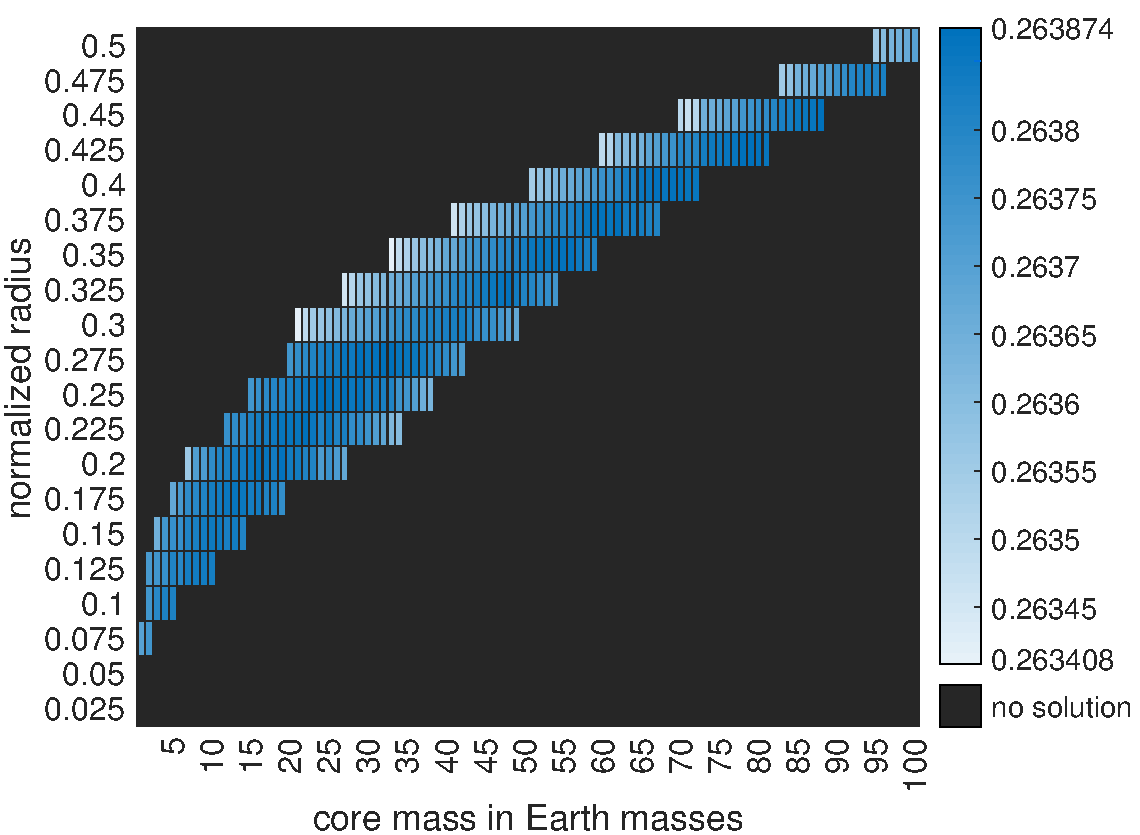
\includegraphics[width = 0.5\textwidth]{Figures/jupiter_area_plotting_MoI_J4.pdf}
    \caption{Summary of all investigated core properties. Each core property combination $m\sub{core}$ \& $r\sub{core}$ is either colored according to the MoI value of its solution or black, if no solution is found. The relative changes of the MoI are in order of 10$^{-3}$. In comparison, the relative changes in $J_2$ and $J_4$ are of the order of 10$^{-5}$ and 10$^{-4}$, respectively. This indicates a dichotomy between the gravitational coefficients and the MoI. By an accurate measurement of the MoI one can eventually further constrain Jupiter's core region and/or density discontinuity in the envelope.\TD{label the colorbar}}
    \label{fig:jupiter_area_plotting_MoI}
\end{figure}

\subsection{The relation between the MoI and the innermost region} \label{subsection:MoI_vs_core}

\begin{table}
\caption{MoI ranges depending on the size and mass of the core and the transition pressure at the density discontinuity in the envelope.}
\centering
 \begin{tabular}{c|c}
%$r\sub{core}$ range & MoI range \\
  MoI range & $r\sub{core}$ range \\
 \hline
0.2634 - 0.26347 & 0.3 - 0.375  \\
0.26347 - 0.26354 & 0.3 - 0.45  \\
0.26354 - 0.26369 & 0.15 - 0.5  \\
0.26369 - 0.26382 & 0.075 - 0.475  \\
0.26382 - 0.26387 & 0.125 - 0.45  \\
%0.075 - 0.175 & 0.26365 - 0.26386  \\
%0.2 - 0.25 & 0.26356 - 0.26387 \\
%0.275 & 0.2651 - 0.26387 \\
\\
$m\sub{core}$ range & MoI range \\
 \hline
0 - 0.025 & 0.26356 - 0.26383 \\
0.025 - 0.06 & 0.26371 - 0.26386 \\
0.06 - 0.11 & 0.2651 - 0.26387 \\
0.11 - 0.24 & 0.26345 - 0.26387 \\
0.24 - 0.32 & 0.26355 - 0.26387 \\
\\
MoI range & $P\sub{trans}$ range \\
 \hline
0.2634 - 0.2636 & 1.5 - 3 \\
0.2636 - 0.26376 & 0.3 - 4.35 \\
0.26376 - 0.26387 & 0.01 - 1.3 \\
 \end{tabular}
\label{tab:MoI:ranges}
\end{table}
As mentioned, the MoI can eventually be used to further constrain the core properties of Jupiter. The upper two parts of table \ref{tab:MoI:ranges} tabulate the results of figure \ref{fig:jupiter_area_plotting_MoI} and list MoI ranges for different core properties, suggesting how an independent measurement of MoI could one day be used to constrain Jupiter's core properties. For example,  
a measurement indicating a large MoI value ($MoI \approx > 0.26355$) would allow a large variety of core properties. But a smaller one ($MoI < 0.26355$) can rule out certain solutions.
To be useful in this way, a measured MoI value must come with relative uncertainty not larger than 0.1\%.
There are different methods to measure and estimate the MoI, e.g., measuring Jupiter's pole precession or the Lense-Thirring acceleration of the Juno spacecraft (\cite{HELLED2011440}).

%Diluted core solutions (above $\sim 0.3~r\sub{core}/R$) yield a 
The shown MoI range of ($MoI \approx 0.2634  - 0.2639$) does not overlap the suggested MoI values of \cite{2017Wahl} ($MoI \approx 0.2640 - 0.2644$). The reason for this discrepancy could be due to different methods of calculation.
The \cite{2017Wahl} results correspond to the CMS method where a lower resolution has been used. In addition, their structure model is based on a physical EoS and therefore has less flexibility in comparison to our polytropic models. 
%These dissimilarities are expected to arise from various calculation methods - they used Concentric Maclaurin Spheroids (CMS) - and their inclusion of higher order $J_{2n}$, although further investigation are necessary. 

\subsection{The relation between the MoI and the density discontinuity in the envelope} \label{subsection:Transition_behavior}
As stated, most density discontinuities occur between $r\sub{trans} \approx 0.75-0.9$ (figure \ref{fig:all_in_one_MoI}, left panel). 
Diluted cores with small MoI tend to have relatively small transition radii ($r\sub{trans} \approx 0.75 -0.79$).
Accordingly, solutions with density discontinuities at large $r\sub{trans}$ tend to have large MoI values. Figure \ref{fig:all_in_one_MoI} (right panel) shows the transition density depending on the transition pressure. The color represents the solution's MoI value. Many density discontinuities occur at a transition pressure of $P\sub{trans} \sim 0.5 - 3 \text{~Mbar}$. Similar to the left panel of figure \ref{fig:all_in_one_MoI} a color trend is observable: Diluted cores with low MoI values tend to have transition pressures $P\sub{trans} \approx 1.5 - 2.7$~Mbar. Lower transition pressures are coupled to higher MoI values and more compact cores. Table \ref{tab:MoI:ranges} summarizes this behavior. \\
These density discontinuities, if confirmed, can be interpreted either as He-rain as proposed by e.g. \cite{Stevenson1975, Stevenson1998}, which is presumed to occur at a pressure region of a few $\sim1$ Mbar (e.g. \cite{Lorenzen2009, Lorenzen2011, Morales2013, Militzer2016, Wilson2010}), leading to a suggested He-depletion (enrichment) in the outer (lower) envelope (e.g. \cite{Guillot1999, Nettelmann2008, Nettelmann2012}. And/Or of the phase transition from molecular to metallic hydrogen which is expected to happen at a similar pressure ($\sim1$ Mbar) (e.g. \cite{Stevenson2013,Helled2018,Mazzola2018}). On the other hand, recent density functional theory simulations, that use the accurate van der Waals density functional, suggest not to have a He rain-out in Jupiter due to its high temperature (\cite{Schottler2018}). An accurate measurement of Jupiter's MoI could constrain the transition regime and therefore test and validate current theories about a possible He-separation or phase transition from molecular to metallic H.  \\ 


\subsection{Polytropes Vs. Polynomials}  \label{subsection:comparison_to_polynomials}
In this work the empirical density profiles are based on polytropes although there are many alternatives. One of which are polynomial-based density structures, that are broadly used in literature as e.g. in \cite{2011Helled, HELLED2011440, Anderson2007}.\\ 
To test and detect potential biases of polytrope-based density profiles, we compare our results (calculated MoI range and density profiles) to polynomial-based solutions. For the latter we use a $8^{\text{th}}$-order polynomial that allows for up to two density discontinuities. To ensure that differences in the results emerge solely from the different methods, the same planet properties, numerical model and calculation method are applied on the polynomial-based calculation. However, polynomial-based solutions are an independent random sample from the posterior in the parameter space and have been found by a Markov-Chain-Monte-Carlo (MCMC) method.
%We use a $8^{\text{th}}$-order polynomial and allow for up to two density jumps. Hence differences in the resulting MoI range and the density profiles represent the differences of the two modeling methods.  
%The results are therefore highly comparable as.
Figure  \ref{fig:histogram} shows the MoI range and distribution resulting from polytropic (left panel) or polynomial (right panel) density structures.
First, the MoI values of both modeling methods are mostly overlapping. Second, also the MoI distribution is almost identical in both panels.
%The MoI distribution of the polytropic-based models is shifted towards larger values. This behavior is confirmed by the polynomial-based models approach. Furthermore, the MoI values of both methods are almost identical. 
Figure \ref{fig:polynomials} shows the resulting distribution of density profiles dependent on Jupiter's normalized mean radius. The solid black line is the ensemble-median and the dashed line mark the 1-sigma width of all density profiles. The color guides the eye and visualizes the width of the distribution.
Obviously the density profiles of polytrope- and polynomial-based structure models are overlapping almost perfectly.
Both, the similarities in the MoI range \& distribution and density profile space reject potential biases in the MoI and structure profiles, legitimizes the choice of polytropes and confirms our results.

\begin{figure*}
    \centering
    \begin{subfigure}{.5\textwidth}
    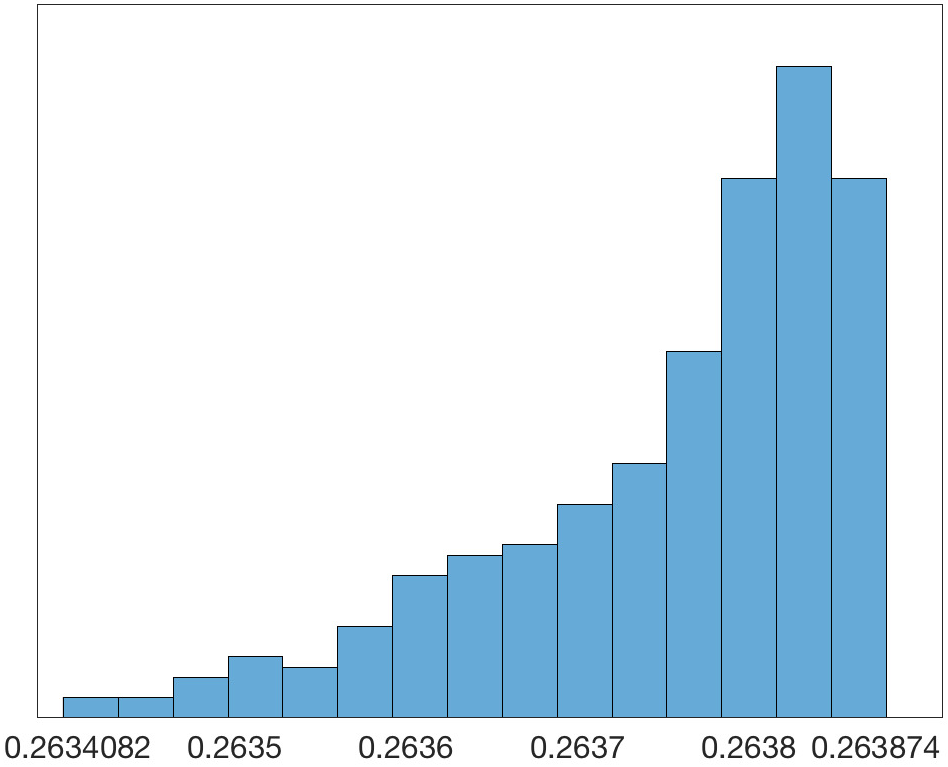
\includegraphics[width = 1\textwidth]{Figures/histogram.pdf}
    \end{subfigure}%
    \begin{subfigure}{.5\textwidth}
    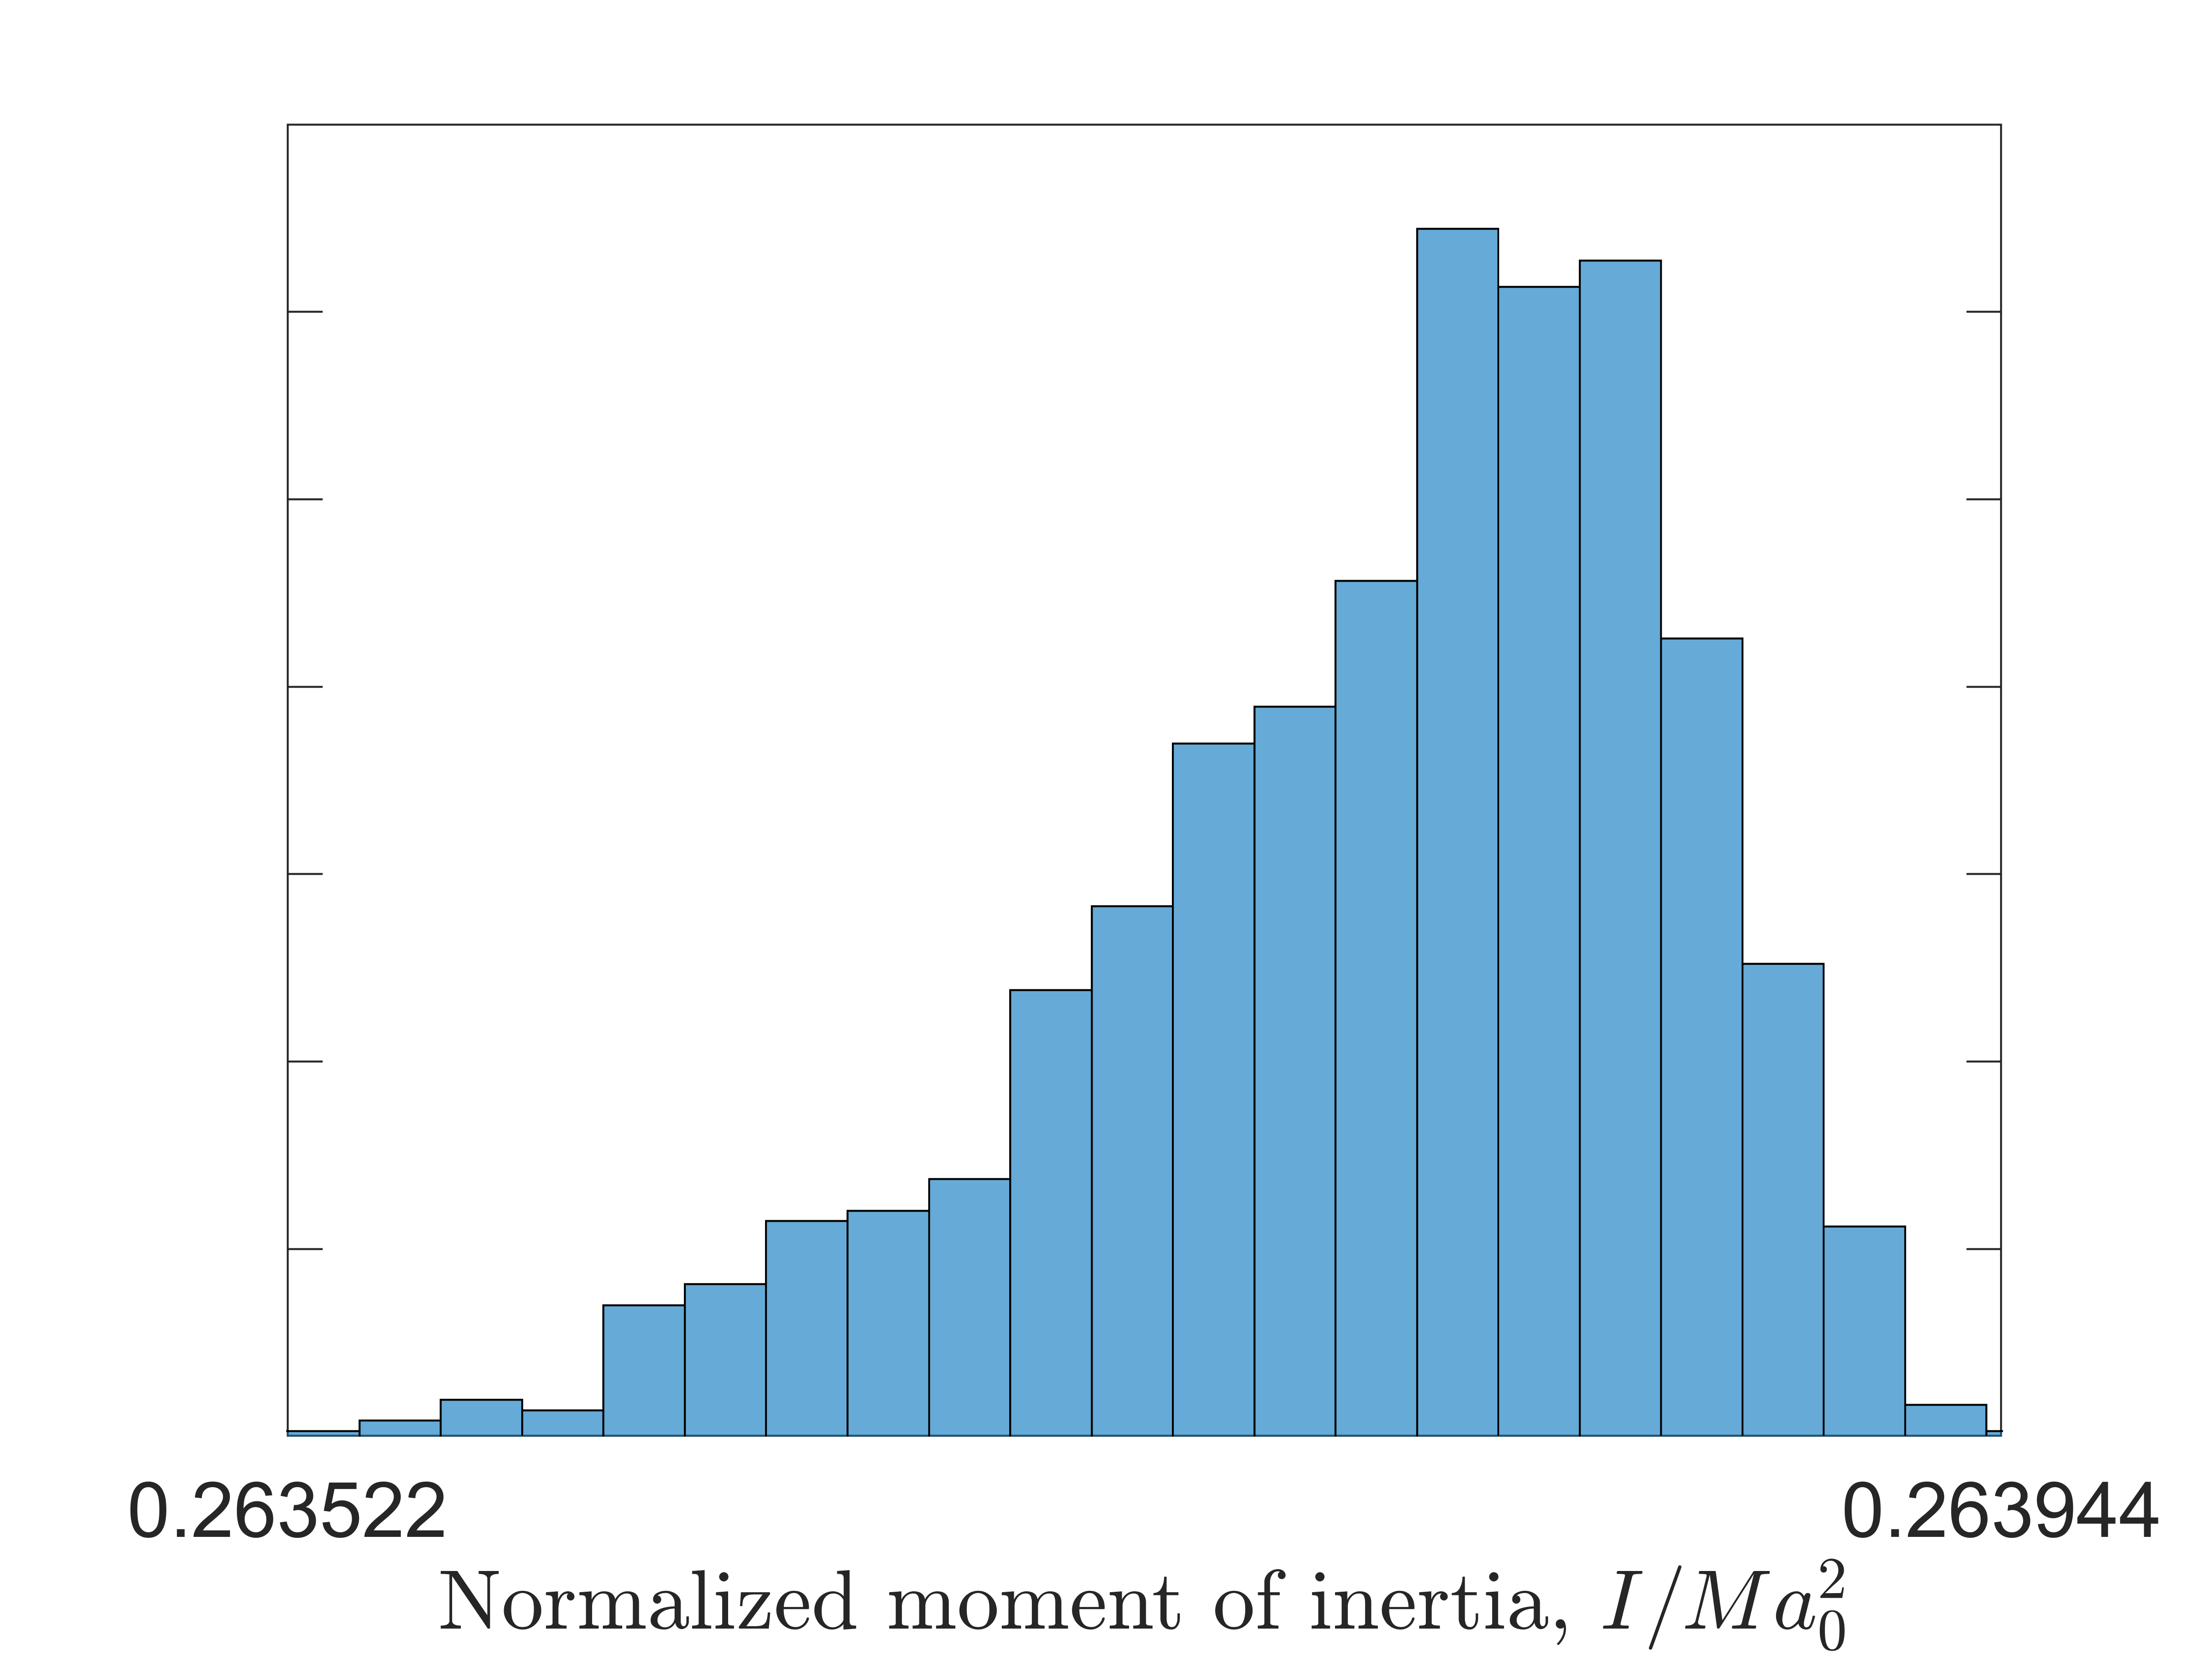
\includegraphics[width = 1\textwidth]{Figures/jupiter_ppwd_4k_d8_J24_I_hist.png}
    \end{subfigure}
    \caption{MoI range and distribution of polytrope-based density structures (left panel) and polynomial-based density structures (right panel). For both modeling methods the ranges and distribution of the MoI almost perfectly overlap. \TD{make same layout for both plots}}
    \label{fig:histogram}
\end{figure*}

\begin{figure}
    \centering
    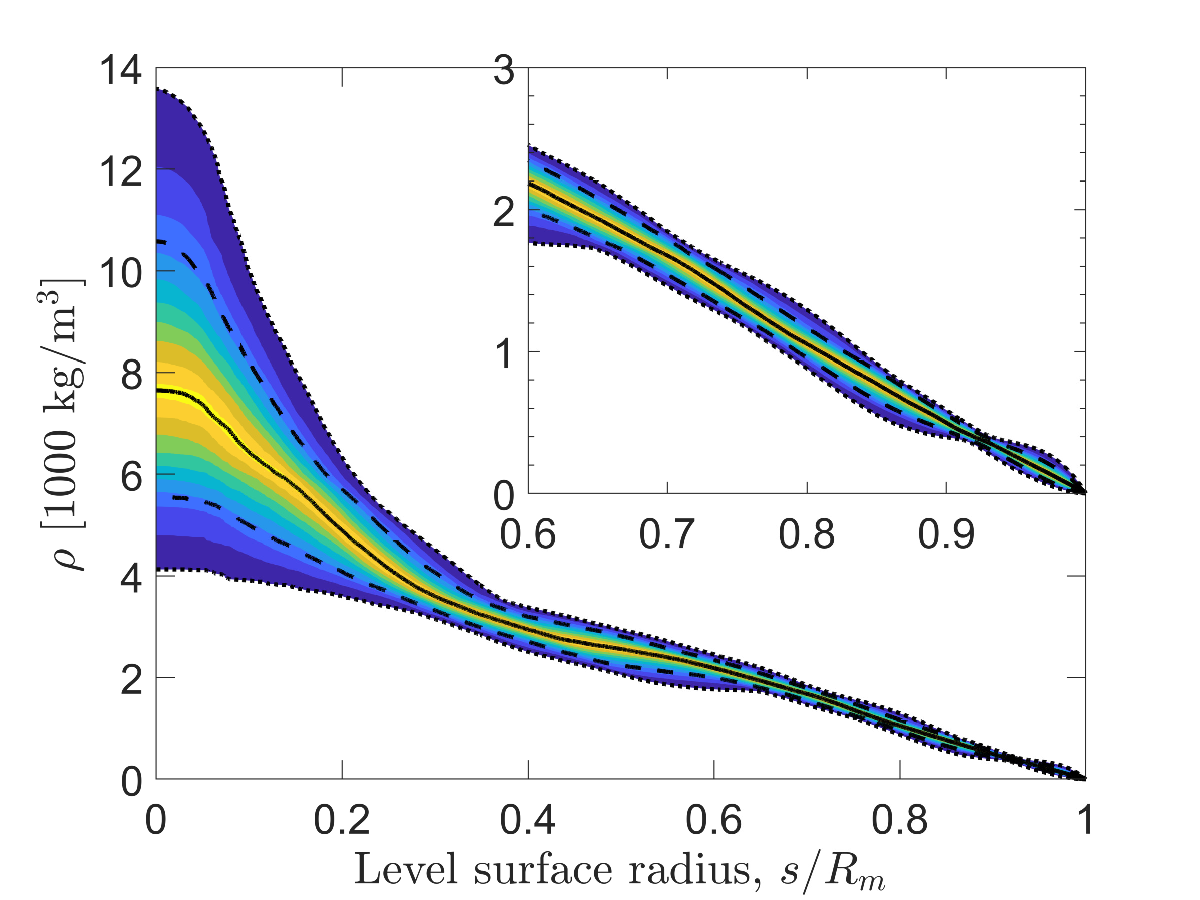
\includegraphics[width = 0.5\textwidth]{Figures/jupiter_ppwd_4k_d8_J24_posterior_average_w_inset.pdf}
    \caption{Distribution of density profiles for Jupiter based on $8^{\text{th}}$-degree polynomials. The black line marks the sample-median and the dashed lines the width of the one-sigma deviation. The color visualizes the sample distribution and comprises 90\% \textbf{(?)} of all solutions. Jupiter's mass, equatorial radius, rotation period, small parameter $m$ and used $J$-values are listed in table \ref{tab:jupiter_properties}. The polynomial-based profiles allow for up to two density jumps and have the same precision as the polytropic-based density structures. Obviously the polynomial-based models cover almost perfectly the same density profile range as the polytropic ones.}
    \label{fig:polynomials}
\end{figure}

\subsection{Resolution Dependent Solutions} \label{subsection:resoltution_dependence}
The computed planetary shape depends on the used precision (i.e., number of equipotential levels). 
As a result, the used resolution affects the inferred gravitational moments and MoI. 
To test the resolution-dependence of $J_2$, $J_4$ and the MoI, we evaluate density profiles of \textit{good results} for various numbers of levels. 
Table \ref{tab:resolution} summarizes the results using an example. The upper (lower) part shows the calculated gravitational coefficients $J_2$ \& $J_4$ and the MoI depending on the number of levels evaluated by ToF (CMS). \\
Independent of the calculation method, the values of $J_2$ \& $J_4$ and the MoI change significant for various numbers of evaluated levels. Nevertheless a convergence is observable for high precision models. To better illustrate this effect, $J$-values that fit the observed gravity data (table \ref{tab:jupiter_properties}) are colored in green. 
%Obviously low resolution models do not fit Jupiter's gravitational moments anymore. 
Obviously it depends on the resolution whether a density profile represents a planets gravity field or not. Accordingly, a low-resolution model converges to a different density profile than a high-resolution solution. This finding is of great importance, as it first limits the comparability of published results based on different resolution. And second a consensus about a minimal resolution has to be reached. For ToF 4$^{\text{th}}$-order we suggest for future studies to evaluate a minimal level number of 1024. For higher resolution, relative changes in $J_2$, $J_4$ and the MoI are in the order of $10^{-4}$ (with respect to the 8192-level result). For CMS no convergence to the method's precision of $10^{-5}$ is found within the tested resolutions. However, to achieve a precision in the order of $10^{-4}$, 4096 levels are necessary. This will set studies on the same base and finally allows to compare nominal results between them. % The more layers are calculated, the more elaborate is a planets density structure, physical shape and evaluated observables.
%Due to different precision the MoI can change in the order of $0.1\%$ which is of the same order as the proposed MoI range (figure \ref{fig:jupiter_area_plotting_MoI} or \ref{fig:all_in_one_MoI}) and the requested precision of a future measurement. 

\begin{table*}
\centering
\caption{$J_2$, $J_4$ and MoI depending on different model resolutions (number of equipotential levels). The evaluated internal structure is fixed for this study and based on a \textit{good result}. The evaluation of the $J$-values and the MoI is done with both ToF (upper part of table) and CMS (lower part of table). Green colored $J$-values are representing Jupiter's gravity field.}
 \begin{tabular}{c|c c c c c}
ToF & 512 & 1024 & 2048 & 4096 & 8192 \\
 \hline
$J_2$ & 0.0146599	&0.0147110	&0.0147021	&\color{green}{0.0146971} &\color{green}{0.0146965} \\
$J_4$ &-0.0005821	&\color{green}{-0.0005864}	&\color{green}-0.0005866	&\color{green}{-0.0005866}	&\color{green}{-0.000586682}\\
MoI	&0.2630856	&0.2637109	&0.2637634	&0.26378450	&0.2638105 \\
\\
CMS & 512 & 1024 & 2048 & 4096 & 8192 \\
 \hline
$J_2$ & 0.0145916	& 0.0146768	& 0.0146851	& 0.0146886 &  0.01469231\\
$J_4$ & -0.0005787	& -0.0005847 & -0.0005856 & -0.0005860 & -0.0005863\\
MoI & 0.2630828	& 0.2637095	& 0.2637627	& 0.2637846 &  0.2638103\\
\\
 \end{tabular}
\label{tab:resolution}
\end{table*}

\subsection{A Constant density vs. a Compressed Core} \label{subsection:CDCvsPC}
Uncertainties in evaluated models do not only depend on the evaluated number of levels but also on the treatment of the core region. 
In this section we investigate the change in the $J_{2n}$ and the MoI values when using a constant density core (CDC) vs. a compressed core (PC) - represented by a polytrope - in a Jupiter-like planet. This planet is not exactly Jupiter but has the same mass, radius and rotation period. To diminish potential effects on $J_{2n}$ and the MoI that are not related to the different core types, we consider only a two-layered density profile (consisting of a core and an envelope) for each core type. For both core models the core mass, core radius and polytropic envelope are the same. Hence the inferred error on the $J_{2n}$ and the MoI represents the differences between the two core types.

Note that we can only fix either the core mass or the core mean density $\Bar{\rho}_{core}$ for both core types, as $M$ and $\Bar{\rho}_{core}$ are related via $\Bar{\rho} = M/V$. 
A system with fixed $\Bar{\rho}_{core}$ and $m\sub{core}$ and total mass M (fixed as a requirement) is over-constrained: A different density distribution changes the planetary shape and therefore its volume. As a consequence, we only present the results for a fixed $m\sub{core}$. Fixing the core average density leads to similar conclusions. \\
To investigate possible effects of the core properties on the inferred errors of $J_{2n}$ and the MoI, we consider five different core densities and envelope polytropes. \\ 
The inferred percentual error is evaluated for different core sizes by using the following equation: 
\begin{equation}
    \text{error} = 100\times \left( \frac{\text{value}_\text{cdc}}{\text{value}_\text{pc}}-1 \right).
    \label{eq:error}
\end{equation}
Figure \ref{fig:Model_comparison} shows the five models color-coded and plotted for a CDC at core sizes of $r\sub{core} = 0.07\, (\text{solid lines}), 0.25\, (\text{dashed lines}), 0.45\, (\text{dotted lines})$. Model 2 represents a massive core, that leads to a large discontinuity at the core-envelope boundary, while Model 5 represents a relatively smooth transitions. The other models represent intermediate cases.

\begin{figure}
    \centering
    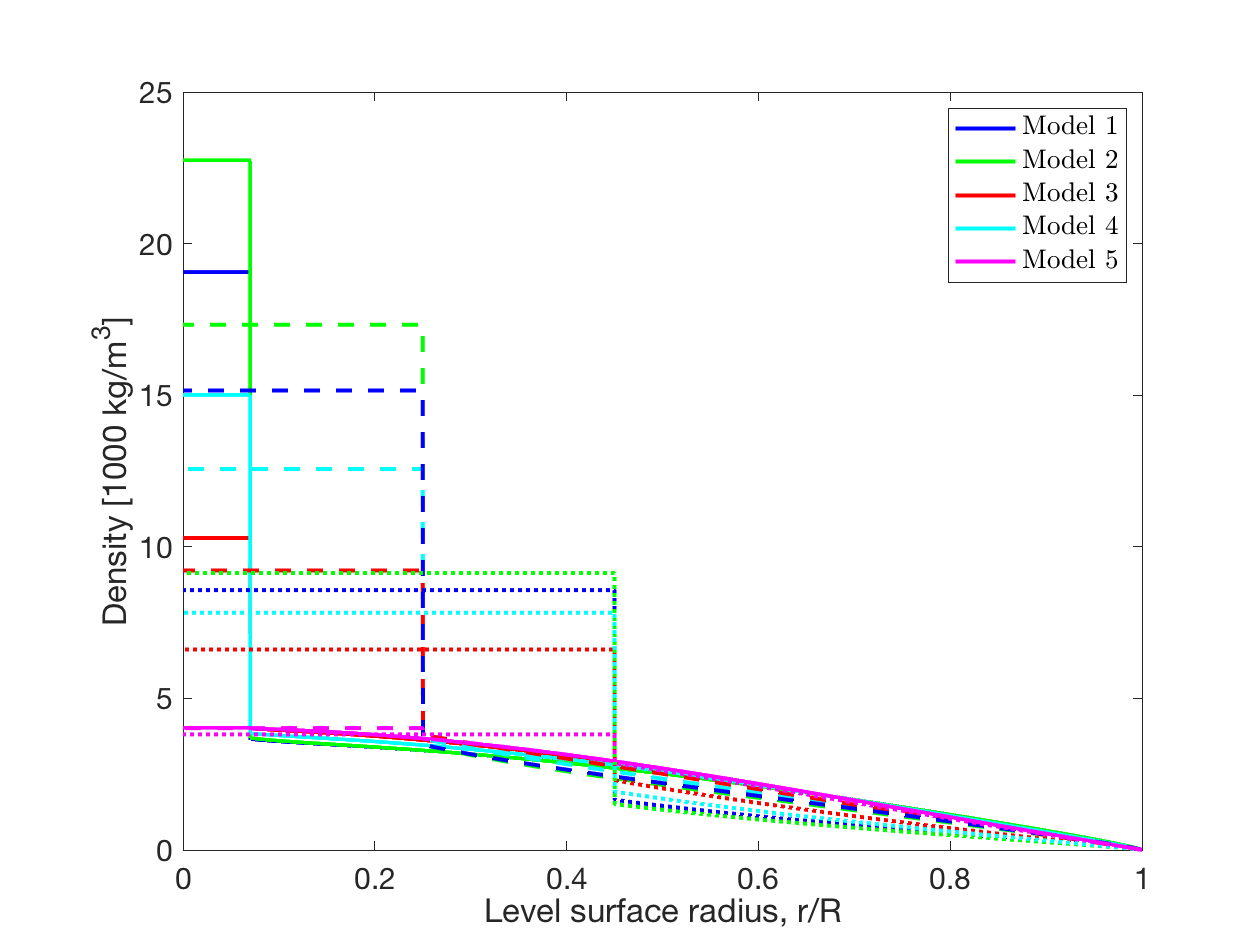
\includegraphics[width = 0.5\textwidth]{Figures/Model_comparison.png}
    \caption{Overview of the five tested CDC models. To generalize the study, five models with different core properties and envelope polytropes are tested. The color shows the different models (only plotted for a CDC) for different core radii: $r\sub{core} = 0.07 (\text{ solid lines}), 0.25 (\text{ dashed lines}), 0.45 (\text{ dotted lines})$. Note that model 2 \& 5 are most extremes with respect to core mass and density jump at the core-envelope boundary.\TD{change names of models}}
    \label{fig:Model_comparison}
\end{figure}

Figure \ref{fig:all_error_J2} shows the percentual differences (denoted as errors) in $J_{2n}$ and the MoI (y-axis) by comparing a CDC with a PC depending on the actual core size (x-axis). 
The colors represent the model (shown in figure \ref{fig:Model_comparison}) and the symbol the corresponding parameter.  
Note that for large core radii $J_2$ is affected the most, mainly followed by the MoI. This seems to be consistent with the contribution functions shown in figure \ref{fig:contr_function} and the Radau-Darwin approximation. However, for small cores, i.e., $r\sub{core} \lsim{0.3}$, the higher-order harmonics are more affected.  
Our interpretation for this behaviour is as follows. 
The gravitational moments are blind to the planet's innermost region (figure \ref{fig:contr_function}). Therefore the inferred errors on the $J_{2n}$ are not generated by the different core types directly. However the core densities of the CDC and the PC are different. This affects the shape and therefore the volume of the whole planet. In return the density profile in the envelope changes. These changes are primarily affecting the higher order gravitational coefficients, due to their relatively large maximal contribution. Hence, for small cores, the inferred errors on the higher order $J$-values are larger than the inferred errors on the lower ones. \\
For core radii larger than a critical core size ($r_{crit}$) the \textit{direct} affection of $J_2$ by the different core types gets dominant. $r_{crit}$ depends on the underlying core model (i.e. its exact mass and density). In our models the critical core size is around $r_{crit}\sim{0.2}$ and therefore in agreement with the contribution functions of \cite{2011Helled}. \\
We find that the error is increasing with increasing core size. As a result, the largest acceptable CDC depends on the demanded precision. Since in this paper we use 4$^{\text{th}}$ order ToF  with a relative precision of $\sim 10^{-4}$, the maximal CDC radius should not exceed $r_{\text{CDC}}\lsim{0.2}$.

Overall, we find that differences between a CDC and a PC strongly depend on the actual core properties. For example, Model 2, which has the highest considered core mass, produces the largest error, in contrast to the smooth (diluted) core of Model 5. \\
%In section \ref{sssec:CDCmcorerhocore} we show that the inferred error strongly depends on the core mass, and the magnitude of the density discontinuity at the core-envelope boundary. Therefore, the maximal acceptable CDC is smaller for more massive and distinct cores (such as Model 2). Further investigations of this topic are desirable and we hope to address them in future research. 
\begin{figure}
    \centering
    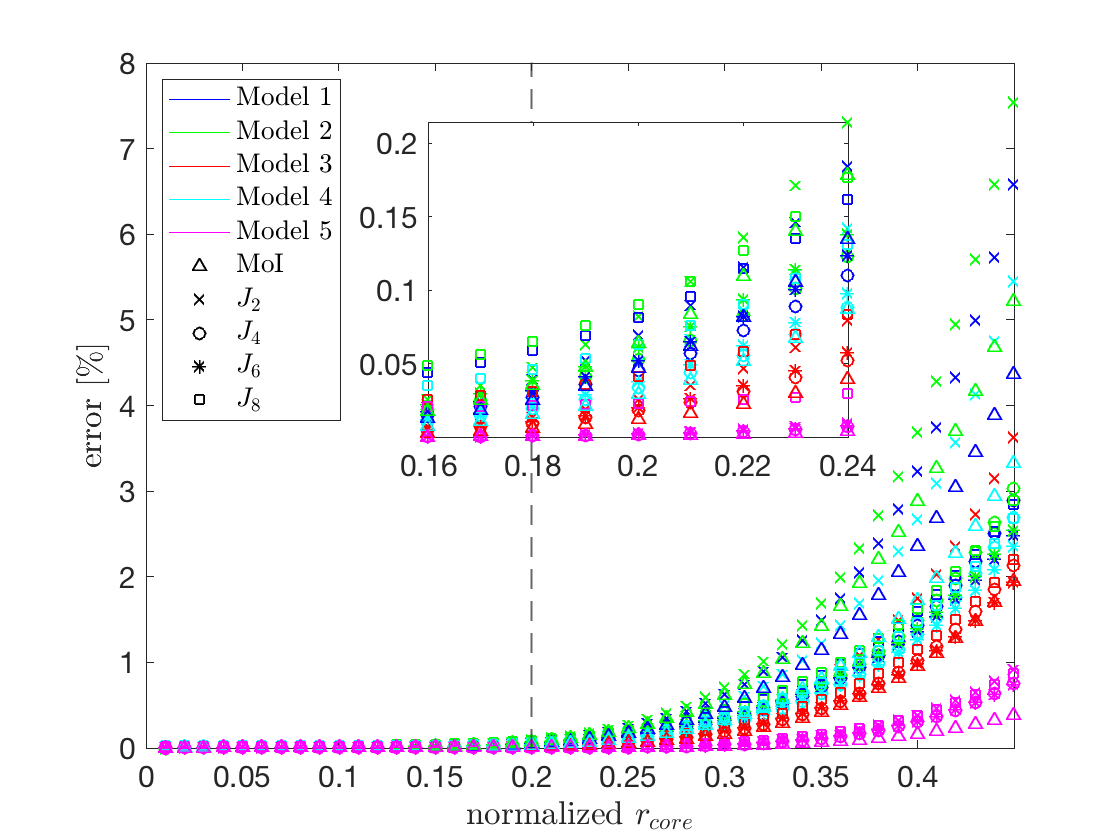
\includegraphics[width = 0.5\textwidth]{Figures/all_kind_of_stuff_in_one.png}
    \caption{Inferred error in the MoI and the $J$-values depending on the core size. Behavior of the error (y-axis), representing the differences in various variables arising by replacing a CDC by a PC, depending on the core size (x-axis). The color represents the different models as shown in figure \ref{fig:Model_comparison}. The the different variables ($J_{2n}$ and MoI) are expressed by various symbols. The dashed line at $r\sub{core}=0.2$ marks the maximum core radius whose inferred error is within the uncertainty of the ToF method.}
    \label{fig:all_error_J2}
\end{figure}
%\subsubsection{affection of core characteristics to $J_2$ and MoI} \label{sssec:CDCmcorerhocore}
We next investigate how $J_2$ and the MoI are affected by the core mass and the magnitude of the density discontinuity at the core-envelope boundary. 
For this analysis we fix the core radius at $r\sub{core}=0.3$ and show for all five models the inferred errors in $J_2$ and the MoI.
Figure \ref{fig:error_vs_mcore} shows the error of $J_{2}$ (blue dots) and the MoI (red dots) on the y-axis, depending on either the core mass (left panel) or the magnitude of the density discontinuity at the core-envelope boundary (right panel) for a fixed core radius of $r\sub{core}=0.3$. 

First we observe that $J_2$ and the MoI are not identical. Neither the points overlap nor the slope does agree (\bncomment{should I draw the lines between the points?}). This confirms again that different information is stored in $J_2$ and the MoI. 
Secondly the inferred error of a low-mass core (or a core with a smooth core-envelope transition) is small. However, this error increases for heavy core masses and distinct density jumps at the core-boundary. This leads us to the expected conclusion that especially the most massive CDC and/or the ones with a very distinct density jump at its core-envelope boundary have to be replaced by a PC. Further investigations of this topic are desirable and we hope to address them in future research. 

\begin{figure*}
    \centering
    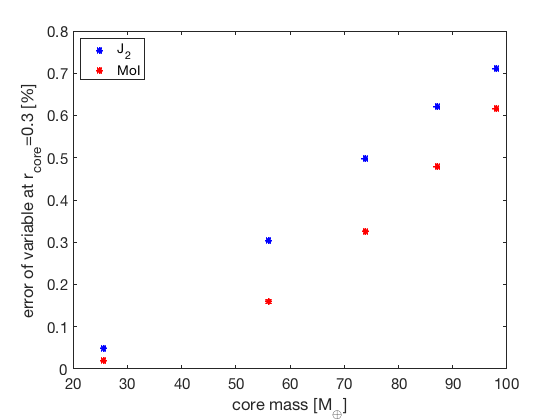
\includegraphics[width = 0.5\textwidth]{Figures/error_vs_mcore_only_J2_MoI.png}%
    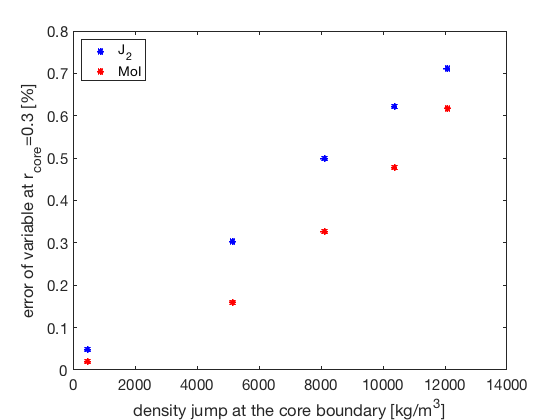
\includegraphics[width = 0.5\textwidth]{Figures/error_vs_densityjump_only_J2_MoI.png}
    \caption{Inferred error in the MoI and $J_2$ depending on either the core mass (left panel) or the density jump at the core envelope boundary (right panel) at a fixed core radius $r\sub{core}=0.3$. We note that neither the inferred errors in $J_2$ and the MoI overlap nor do the curve slopes agree. This confirms again that different information is stored in  $J_2$ and the MoI. The inferred errors in $J_2$ and the MoI are smaller for low mass cores and for (diluted) cores with rather smooth core-envelope transitions. Therefore especially massive and distinct CDC have to be replaced by a PC.}
    \label{fig:error_vs_mcore}
\end{figure*}

\section{Discussion, Summary and Future Work}\label{sec:summary}
We present empirical density profiles of Jupiter, represented by up to three polytropes, that fit Jupiter's mass, equatorial radius, rotation rate and the observed second and fourth gravitational constant $J_2$ and $J_4$. The density profiles are evaluated by ToF. The presented approach is facing some weaknesses which will be discussed here. \\
First the ToF calculation method cannot account for differential rotation and asymmetries between the hemispheres. However, we respect the contribution of the winds in the uncertainties of $J_2$ and $J_4$. Second, polytropes are not appropriate to describe Jupiter's surface density as measured by the Galileo Entry Probe. In fact polytropes struggle to reproduce low surface densities. Admittedly, this effect is supposed to be small as it only concerns Jupiter's outermost 0.5 M$_\oplus$ and its surface density is barely captured by $J_2$ and $J_4$ but mostly effects higher-order $J$-values. Further, polynomial-based structure models that account for Jupiter's measured surface density yield similar results with respect to the MoI range and density profiles. Still and all, the Galileo entry probe could only resolve one small spot at Jupiter's dynamical atmosphere, hence an extrapolation to its whole atmosphere has to be treated with caution. The atmospheric density structure is thought to change over time, this puts additional uncertainties to Jupiter's surface structure. Finally the presented density profiles are only converged to $J_2$ and $J_4$. More accurate model evaluations including higher order gravitational harmonics are highly valuable and subject of current research. 
%However higher order $J$-values are more sensitive to the outermost region of Jupiter, barely affecting the 

We then analyze the empirical density profiles to first investigate the dependence between $J_2$, $J_4$ and the MoI and applied it on various core properties. Next we explore under what condition the MoI further constrains the core region and/or the predicted He-separation in the envelope. Then we investigated the effect of the model resolution (e.g., numbers of equipotential levels) on $J_2$, $J_4$ and the MoI and compared our polytrope-based structure models to polynomial-based models. Finally, the effect of a CDC simplification on the precision of the gravitational coefficients and the MoI is investigated. For that purpose a only two-layered Jupiter-like planet is used. \\
%By using polytropes, no composition assumption has to be made, resulting in a unbiased approach of describing Jupiter's interior. The core properties are constraint to $r_{core, max} = 0.4$, $m_{core, max} = 60 \text{ M}_\oplus$ and $\rho\sub{max} = 32'000 \text{ kg/m}^3$. \\
Our main conclusions can be summarized as follows:

\noindent

\begin{itemize}[
  align=left,
  leftmargin=1.4em,
  itemindent=0pt,
  labelsep=0pt,
  labelwidth=1.4em
]
\item We show in several ways that the MoI is not identical to $J_2$ as proposed by the Radau-Darwin approximation. There is different information contained in an accurately measured MoI than in the gravitational coefficients $J_2$ and $J_4$. 

\item Our proposed MoI value ranges from $0.263408 - 0.263874$ giving relative (absolute) changes in the order of $10^{-3}$ ($10^{-4}$).
If the MoI is measured with a relative precision better than 0.1\%, it potentially can constrain Jupiter's core and/or the transition properties of the density discontinuity in the planet's envelope (table \ref{tab:MoI:ranges}). Such features are possibly caused by He-separation and/or H metallization.
%(figure \ref{fig:all_in_one_MoI}, right panel)
% while $J_2$ and $J_4$ are measured to a relative accuracy of $10^{-5}$? and $10^{-5}$?, respectively.
%\item We suggest to observe features of helium rain, as without constrains, density jumps in the envelope often happens at radii $\sim 0.75-0.9r/R$? and at pressures $\sim 0.5-3\,\text{ Mbar}$.

\item We confirmed our results based on polytropic density structures with structures based on $8^{\text{th}}$-order polynomials. 
%To legitimate and test our polytrope-based empirical structure models on potential biases, we compared the MoI-value range and distribution and the density profiles to solutions based on a $8^{\text{th}}$-order polynomial. 
%We conclude that t
The range and distribution of MoI values are almost identical (figure \ref{fig:histogram}) and the density profiles of both modeling methods are almost perfectly overlapping (figure \ref{fig:all_in_one_MoI} \& \ref{fig:polynomials}). 
This legitimates and strengthens the polytropic-based density structures as it rejects potential limitations or biases in the solution-space. 

\item %We investigated model resolution effects on $J_2$, $J_4$ and the MoI. For that a fixed structure model was evaluated with various layer numbers. 
We noticed that $J_2$, $J_4$ and the MoI values depend on the used model resolution but converge for a higher level number. We suggest for ToF a minimum resolution of 1024. For CMS no convergence to its relative methodical precision of $10^{-5}$ is observed within the investigated resolution. But to achieve a similar precision as ToF, a level number of 2048 is necessary.

\item A CDC of a Jupiter-like planet should not exceed the size of $r\sub{core} = 0.2$. Any larger CDC generates inferred errors in $J_{2n}$ and in the MoI larger than $~10^{-4}$, that corresponds to the relative uncertainty of ToF. \\
However the inferred error depends strongly on the core properties:
    \begin{enumerate}[leftmargin=0.3cm, labelwidth = 0cm, itemindent=0cm,labelsep = 6pt]
        \item[$-$] the more massive the core, the larger the inferred error 
        \item[$-$] the more distinct the density discontinuity at the core-envelope boundary, the larger the inferred error
    \end{enumerate}{}
    
%\item The inferred error of a small and low-density CDC with a smooth core-envelope transition is mostly seen in the higher order $J_{2n}$ as they get perturbed indirectly via the change of shape of the core and therefore the planet. \bncomment{I think I can delete this point?!}

\end{itemize}

%\subsection{Future}
It should be noted that this study represents only the beginning, and further research should follow. 
%of a more rigorous analysis of the giant planets in the Solar System. Further investigations are needed in the manner of completeness, statistics (?) and interpretation. A non-complete list of successive studies is presented below:
%\begin{itemize}
 %   \item 
First, this research was conducted using a 4$^{\text{th}}$ order ToF. It is desirable to refine all calculations with the method of CMS, as it is more expensive but also more precise. 
Second, since we concentrated on the relation between $J_2$, $J_4$ and the MoI our models were designed to fit Jupiter's measured $J_2$ and $J_4$. It would be valuable to produce density profiles that fit the gravity data beyond $J_4$, %\bncomment{although the MoI range will not be constrained by doing so (Naor test)}. 
In addition, to get the most complete results, a global minimum search function should be used. 
Finally, we suggest that the inferred density profiles, which in fact provide the density-pressure relation in Jupiter should be interpreted in terms of composition and its depth dependence using physical equations of state. We hope to address these topics in future research. 
% The effects of a CDC and PC on the precision of important variables has to be generalized to even more extreme core properties and more planets (different masses, radii and rotation periods).

\section{Acknowledgments}

\scalefont{0.94}
\setlength{\bibhang}{1.6em}
\setlength\labelwidth{0.0em}
\bibliographystyle{mnras}
\bibliography{references}
\normalsize

\appendix
\section{Proof of concept}
To proof the used version of Theory of Figures 4$^{th}$ order, different benchmarks and comparisons to other methods are presented. 
First we benchmark the normalized moment of inertia of a non-rotating planet consisting of one polytrope evaluated by our ToF method to the results of \cite{Lattimer_2001}. Table \ref{tab:comp.MoI} lists for various index-values ($n$-values, eq. \ref{eq:polytrope}) the evaluated solution of our ToF method, the solution by \cite{Lattimer_2001} and the relative difference between them. The relative error is found not to exceed $10^{-4}$. 
Second the density profile of a non-rotating planet consisting of one polytrope is compared to its analytical solution. Figure \ref{fig:test_non_rot_density_profile} shows the normalized density depending on the normalized planetary radius. The dashed green line marks the analytical solution while the solid black line represents the calculated profile consisting of 4096 equipotential levels. Normalization factors are given in the figure, where $G$ is the gravitational constant, $K$ the polytropic constant and $M$ the total mass of the planet. Note that both solutions are almost identical.
Finally, a polytrope-1-index planet is evaluated by ToF consisting of 4096 levels and the resulting $J_2$ and $J_4$  are compared to results proposed by other methods and studies. Table \ref{tab:comp.J2J4} lists $J_2$ and $J_4$ values evaluated by our ToF method, CMS method consisting of 512 levels (by \cite{Hubbard_2013}), the exact Bessel solution (eBe) and Consistent Level Curve (CLC), both by \cite{Wisdom_2016}. Relative differences in $J_2$ and $J_4$ between ToF and the other methods are in the order of $10^{-4}$.

\begin{table}
\centering
 \begin{tabular}{c| c c c}
$n$ & ToF & \cite{Lattimer_2001} & rel. difference \\
 \hline
0.5 & 0.32587  & 0.32593 & 1.72$*10^{-4}$ \\
1.0 & 0.26139 & 0.26138 & 3.83$*10^{-5}$ \\
2.0 & 0.15497 & 0.15485 & 7.58$*10^{-4}$ \\
 \end{tabular}
\caption{The MoI of a non-rotating planet depending on various polytropic indices ($n$), evaluated by either ToF (left column) or proposed by \cite{Lattimer_2001} (middle column). To benchmark our used ToF method, the relative differences in the MoI values for each $n$ is shown in the third column. It is found that the precision of our ToF method does not exceed $10^{-4}$. }
\label{tab:comp.MoI}
\end{table}

\begin{table}
\centering
 \begin{tabular}{r| c c c c}
 & ToF & CMS-512 & eBe & CLC \\
 \hline
$J_2*10^2$ & 1.39955 & 1.39892 & 1.39885 & 1.39885 \\
$-J_4*10^4$ & 5.32240 & 5.31880 & 5.31828 & 5.31828 \\
 \end{tabular}
\caption{$J_2$ and $J_4$ of a index-1-polytrope evaluated by either our ToF method, CMS (by \cite{Hubbard_2013}), the exact Bessel solution (eBe) and Consistent Level Curve (CLC) both by \cite{Wisdom_2016}. Relative differences between our ToF method and the other methods are not larger than $10^{-4}$.}
\label{tab:comp.J2J4}
\end{table}

\begin{figure}
    \centering
    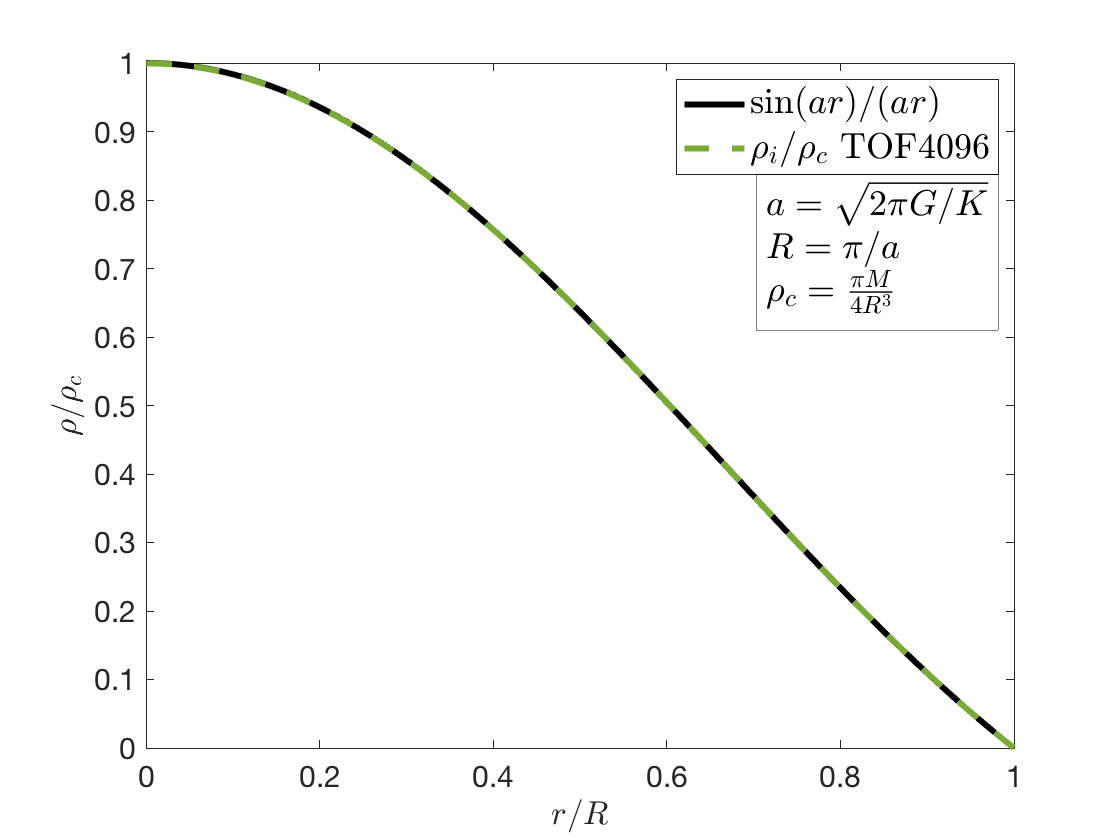
\includegraphics[width = 0.5\textwidth]{Figures/test_non_rot_density_profile.png}
    \caption{Bench-marking the ToF calculation method to an analytical solution of a non-rotating index-1-polytrope. The density profiles, either evaluated analytically (black solid line) or with ToF (green dashed line), are overlying almost perfectly. Deviations are in the order of $10^{-4}$.}
    \label{fig:test_non_rot_density_profile}
\end{figure}

\begin{figure}
    \centering
    \includegraphics[width = 0.5\textwidth]{Figures/jupiter_all_in_one_P_of_rho_J4.pdf}
    \caption{All barotropes (pressure depending on the density) of \textit{good results} collected in one figure. Profiles are colored according to the model's MoI. The black curve shows the barotrope proposed by \cite{Miguel2016}, whereas the black dotted and dash-dotted lines mark the solution of \cite{Debras_2019} and the one of a index-1-polytrope, respectively. The external profiles are in good agreement, although the solution of \cite{Debras_2019} marks an upper (lower) pressure boundary at densities around $1500\,$kg/m$^3$ ($2800\,$kg/m$^3$). 
    %Further our solutions underestimates Jupiter's surface density in the outermost radial 1\%. This issue however resolves by considering higher order J-values. 
    %Note that polytropes struggle to represent the outermost 1\% of Jupiter's radius.
    }
    \label{fig:all_in_one_P_of_rho}
\end{figure}

\section{barotropes}
Figure \ref{fig:all_in_one_P_of_rho} shows pressure profiles depending on the density of all \textit{good results}. The color is representing the MoI-value of each solution. The solid, dotted and dash-dotted black lines mark solutions of \cite{Miguel2016}, \cite{Debras_2019} and an index-one-polytrope, respectively. Obviously the external profiles are in agreement with our solution space, although the result of \cite{Debras_2019} clearly marks an upper (lower) pressure bound at a density of $\sim{1500~\text{kg/m}^3}$ ($\sim{2800~\text{kg/m}^3}$). \\
\TD{rename the Models 1-5 with more physical names, change order of naming} \\
\TD{maybe change PC to CC (compressed core)} \\
%\TD{add this in the discussion?:} \\
%Although density profiles are truncated to a maximal density of $\rho\sub{max}=32'000 \text{ Kg/m$^3$}$, a more careful treatment is necessary to discard unrealistic density profiles not only in the matter of maximal density but also with respect to the density gradient. For small but heavy cores a steep density gradient within the core may arise. Very precipitously slopes can not be explained by pure compression of material (as not even hydrogen is compressible by that extend) but solely with a compositional gradient. A reasonable choice of a composition gradient and its corresponding slope is subject of current research.

\bsp %typesetting comment
\label{lastpage}
\end{document}
